
\chapter{Data Quality and Initial Exploratory Assessment}\label{appendix:data_quality}
	
\section{Data Quality Assessment}

Prior to conducting business intelligence analysis, the advertising campaign dataset was evaluated to ensure its quality, reliability, and suitability for analysis. The objective of this assessment is to identify potential data quality issues, validate the performance metrics used throughout the project, examine unusual observations, and establish a set of baseline metrics that will guide subsequent business analysis.

The dataset contains daily advertising campaign performance across multiple platforms, regions, target audiences, product categories, and creative types during the first quarter of 2024.
	
	
	
	
\subsection{Data Type}

The data types of all variables were first examined to verify that each column was stored using an appropriate data type. As shown in\textit{ Fig. \ref{fig:check_datatype}}, numerical variables were stored as either \texttt{int64} or \texttt{float64}, categorical variables as \texttt{object}, the \texttt{Date} column as \texttt{datetime64[ns]}, and the \texttt{Is\_Competitive\_Event} variable as a boolean. 

\begin{figure}[h]
	\centering
	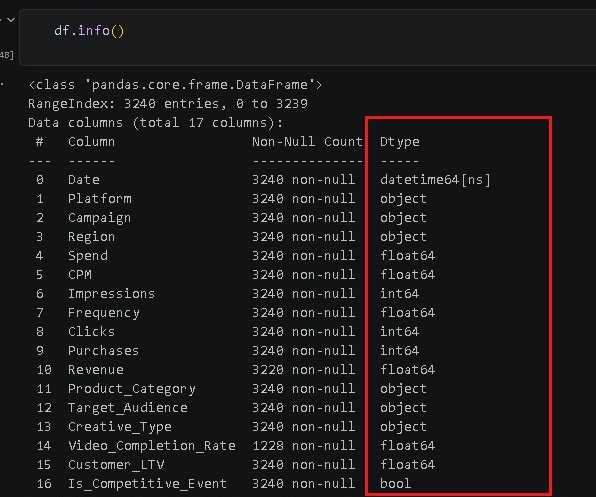
\includegraphics[width=0.45\textwidth]{images/check_datatype.jpg}
	\caption{Checking datatypes of the dataframe}
	\label{fig:check_datatype}
\end{figure}
No inconsistencies in data types were identified; therefore, no type conversions were required.

\subsection{Duplicate Records}

The dataset was examined for duplicate observations.

\begin{figure}[h]
	\centering
	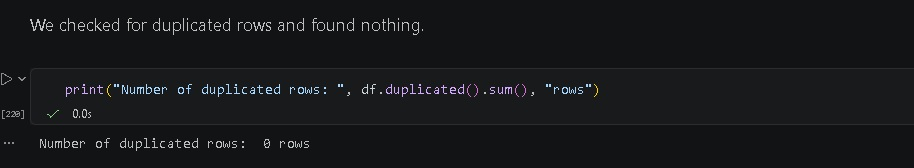
\includegraphics[width=0.8\textwidth]{images/duplicate_records.jpg}
	\caption{Checking for duplicate records}
	\label{fig:duplicate_records}
\end{figure}


No duplicate records were identified as shown in \textit{Fig. \ref{fig:duplicate_records}}.



\subsection{Data Completeness}

The dataset was examined for missing values to determine whether incomplete observations could affect subsequent analyses.

\begin{itemize}
	
	\item \textbf{Revenue}
	
	A sample of these datapoints are shown in \textit{Fig. \ref{fig:missing_values}}. It can be seen that twenty observations (approximately 0.6\% of the dataset) contained missing revenue values.
	\begin{figure}[h]
		\centering
		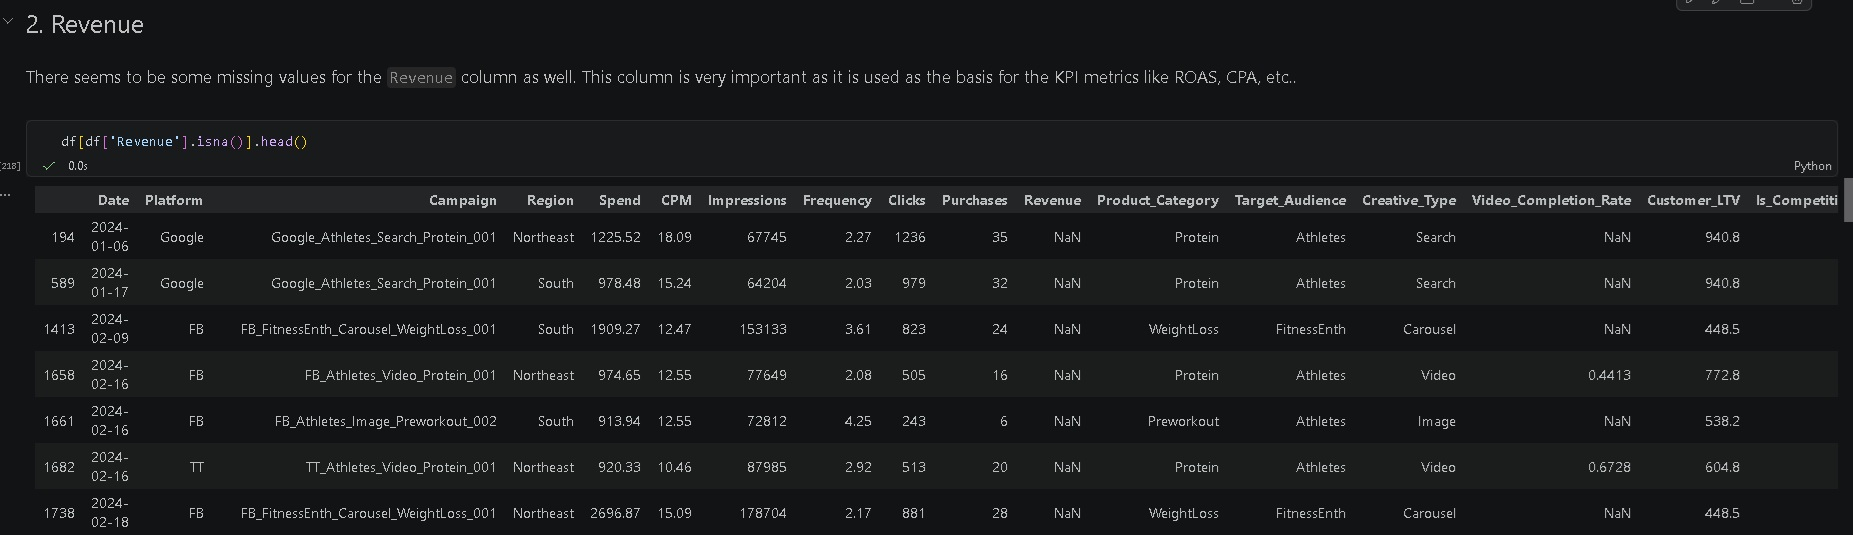
\includegraphics[width=1\textwidth]{images/revenue_missing_values.jpg}
		\caption{Sample datapoints with missing revenues.}
		\label{fig:missing_values}
	\end{figure}



	
	Because these represented a very small proportion of the data and no systematic pattern of missingness was identified, the corresponding observations were removed as shown in\textit{ Fig. \ref{fig:drop_missing_values}} prior to analysis.
\begin{figure}[h]
	\centering
	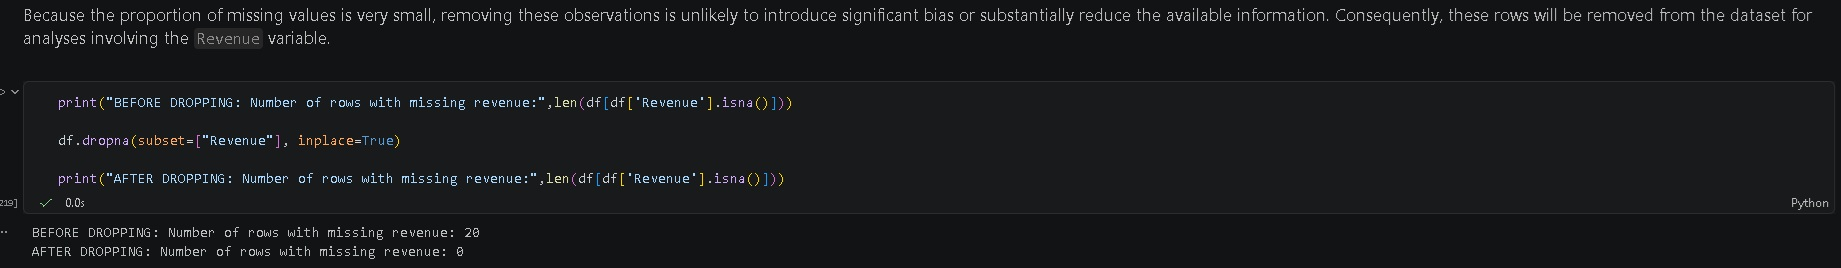
\includegraphics[width=1\textwidth]{images/drop_missing_revenue.jpg}
	\caption{Dropped datapoints with missing revenues.}
	\label{fig:drop_missing_values}
\end{figure}
		
	
	\item \textbf{Video Completion Rate}
	
	A large number of missing values were initially observed in the \textit{Video Completion Rate} variable. Around 62\% of the total dataset! 
	
\begin{figure}[h]
	\centering
	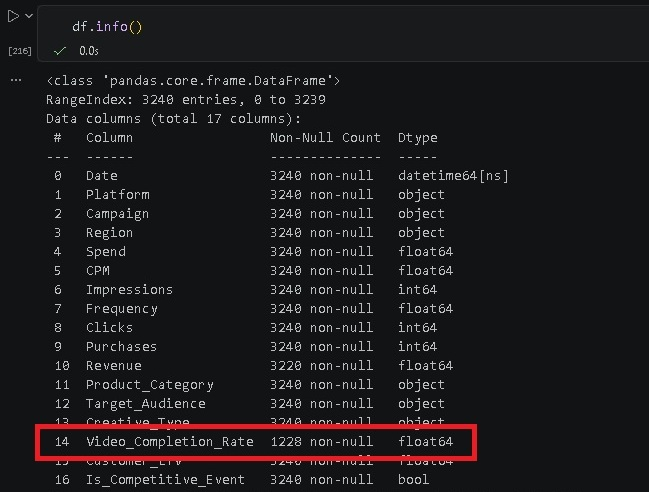
\includegraphics[width=0.45\textwidth]{images/video_completion_missing.jpg}
	\caption{\texttt{video\_completion\_rate} missing values}
	\label{fig:video_completion_missing}
\end{figure}
	
	
	
	
	Further investigation revealed that this metric is only applicable to \textbf{campaigns using video advertisements}. After restricting the dataframe to video creatives, \textbf{only 212 missing observations remained} as shown in \textit{Fig. \ref{fig:filtered_video_completion_missing}}. 
	
\begin{figure}[h]
	\centering
	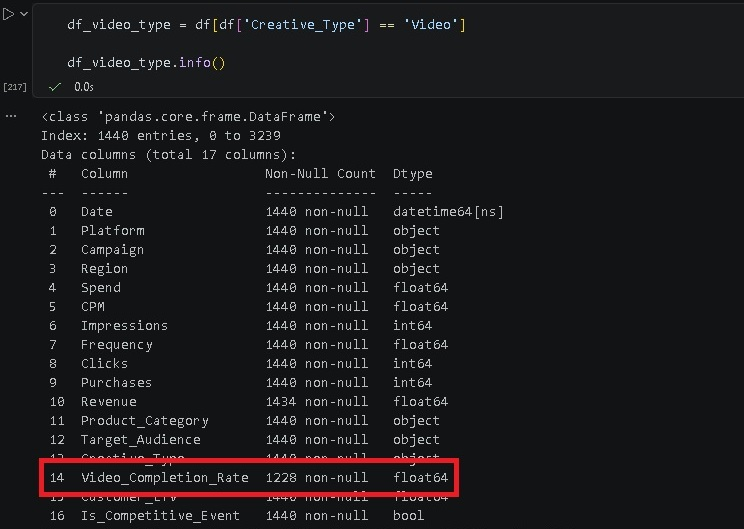
\includegraphics[width=0.45\textwidth]{images/filtered_video_completion_missing.jpg}
	\caption{DataFrame filtered to video creative types}
	\label{fig:filtered_video_completion_missing}
\end{figure}	
	

	Consequently, these missing values were treated as \textbf{structurally missing} rather than data quality issues, and analyses involving this variable will use only the relevant subset of campaigns.
	
\end{itemize}

	\subsection{Logical Consistency Checks}
	
	Several validation checks were performed to identify logically inconsistent observations.
	
	\subsubsection{0 Clicks with non-zero purchase}
	
	I noticed that there were rows with 0 clicks but has non-zero Purchases, which I thought was weird at first. How are they able to purchase without clicking the ad. 
	
	Apparently, this happens in real world scenarios and they are called \textbf{view-through conversions}. People see the ad, they don't click it then later that evening, they remembered the brand and typed the website into google and bought the product.
	
	\begin{figure}[h]
		\centering
		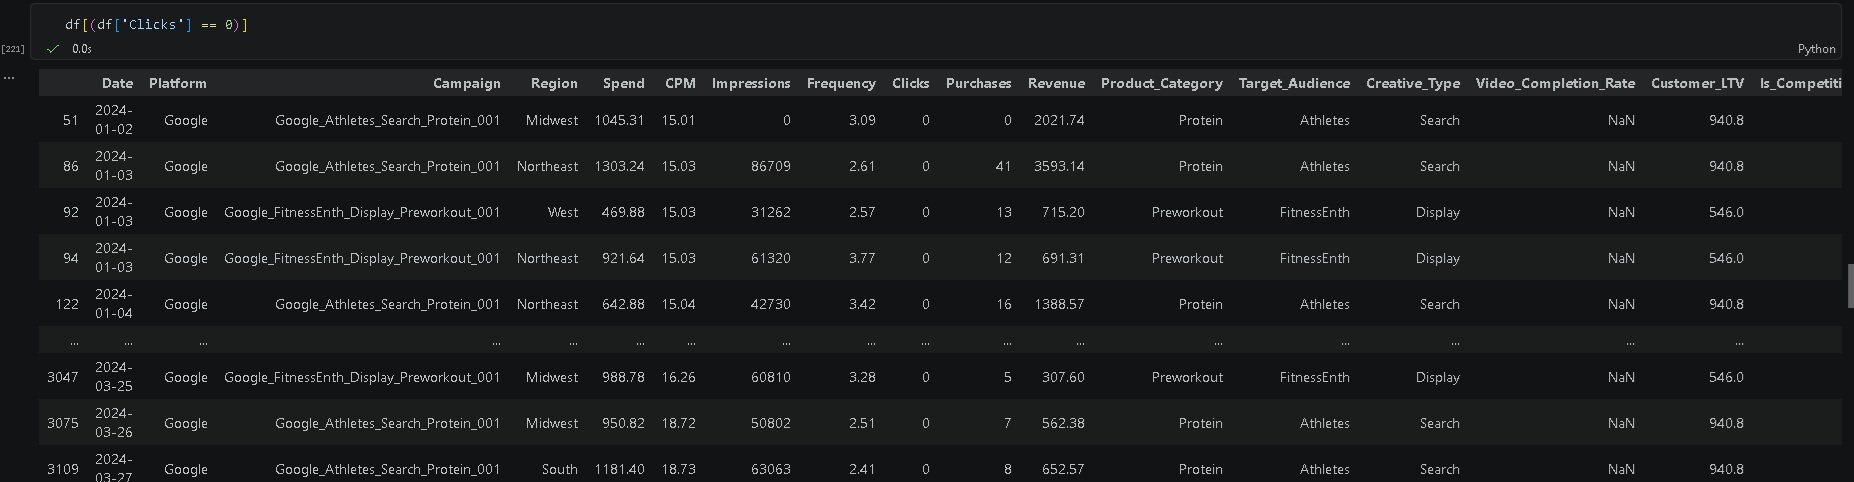
\includegraphics[width=0.8\textwidth]{images/0clicks_non0purchase.jpg}
		\caption{Sample datapoints with 0 clicks but non-zero purchase}
		\label{fig:0clicks_non0purchase}
	\end{figure}
	
	
	But, at this point, I was wondering how they know which ad actually influenced the purchased without click or what if the buyer interacted with multiple ads before purchasing(cross-channel conversions). Apparently, this is related to \textbf{attribution}, and there are multiple attribution models like \textbf{last\_click attribution}, \textbf{first-click attribution}, \textbf{linear\_attribution}, etc.. which is not part of this data cleaning process. 
	
	So, for now, I'll just assume that this dataset was collected using a certain attribution model and leave it at that. This justifies the 0 clicks with non-zero purchase.
	
\begin{tcolorbox}
	\textbf{Side Note:} After the data cleaning, all rows with zero clicks belong to the Google platform. (For the time being, this is just an observation. I'm noting it here so I don't forget to investigate it later.)
\end{tcolorbox}
	
	\subsubsection{0 Impressions with non-zero Cost-Per-Mile(CPM)}
	
	Cost Per Mille (CPM) measures the advertising cost required to generate 1,000 impressions and is commonly used to evaluate the cost efficiency of awareness campaigns.
	
	\begin{equation}
		\text{CPM} = \frac{\text{Spend}}{\text{Impressions}} \times 1000
	\end{equation}
	
	Because impressions appear in the denominator, CPM is undefined when the number of impressions is zero.
	
	During the data quality assessment, 47 observations (approximately 1.45\% of the dataset) were identified with \texttt{Impressions = 0} but non-zero with CPM values. 
	

	Furthermore, all of these observations originated from the Midwest region as shown in \textit{Fig. \ref{fig:0impression}}, suggesting a systematic reporting inconsistency rather than isolated data entry errors.
	
	\begin{figure}[h]
		\centering
		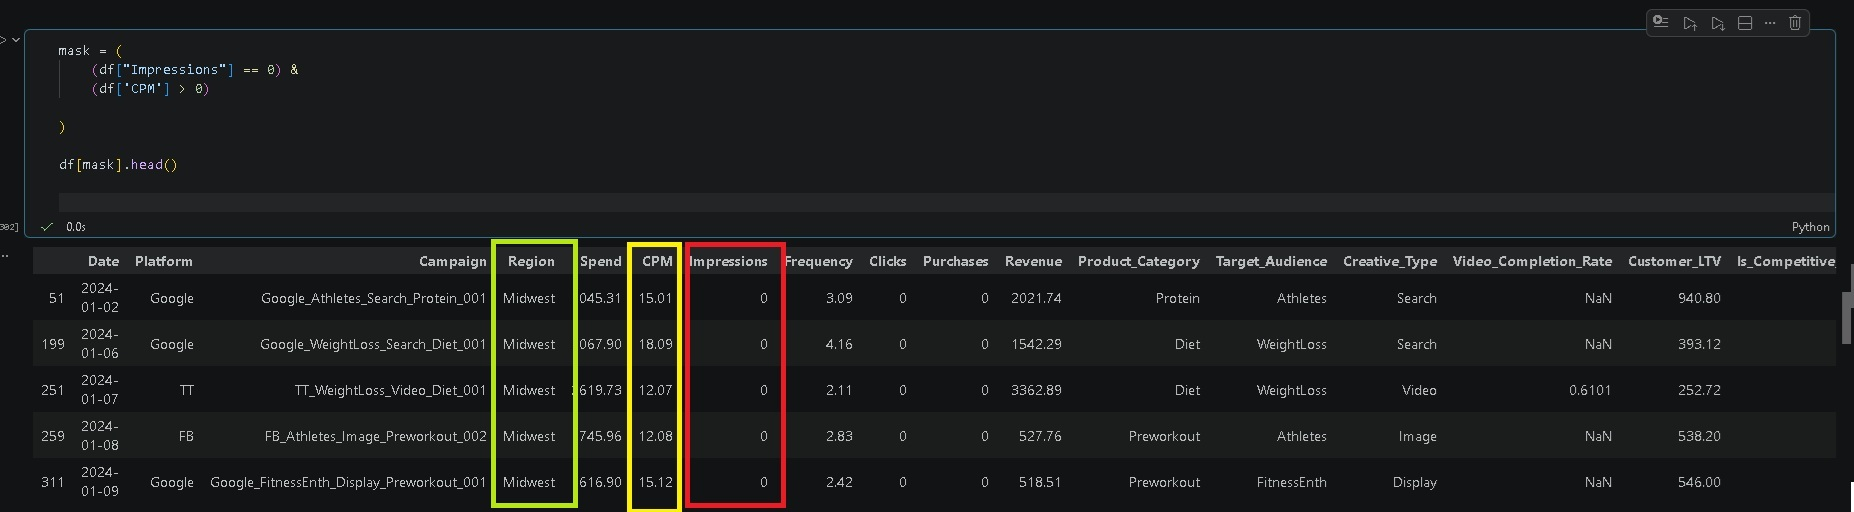
\includegraphics[width=0.8\textwidth]{images/0impressions.jpg}
		\caption{Sample rows that has 0 impressions with non-zero CPM}
		\label{fig:0impression}
	\end{figure}
	
	
	Since these observations violate the definition of CPM and the 0 impressions value could affect the calculation of other performance metrics, such as CTR and CVR, they were removed from the dataset prior to analysis.
	
	\begin{figure}[h]
		\centering
		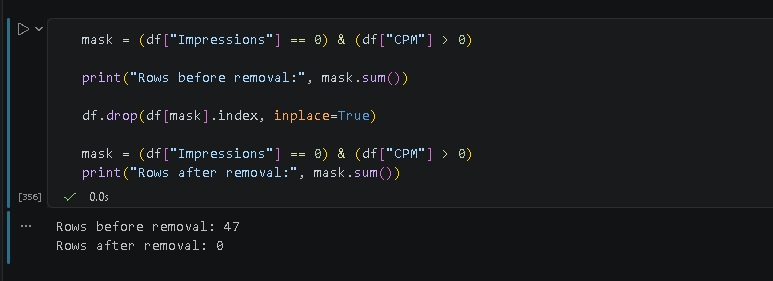
\includegraphics[width=0.8\textwidth]{images/0impressionscount.jpg}
		\caption{Dropped Rows that has 0 impressions with non-zero CPM}
		\label{fig:0impression_count}
	\end{figure}
	
		\subsection{Outlier Assessment}
	Boxplots were used to identify potential outliers across the numerical variables as shown in \textit{Fig. \ref{fig:box_plots}}. Severe outliers were identified for the Spend column and will be investigated in this section.
	\begin{figure}[h]
		\centering
		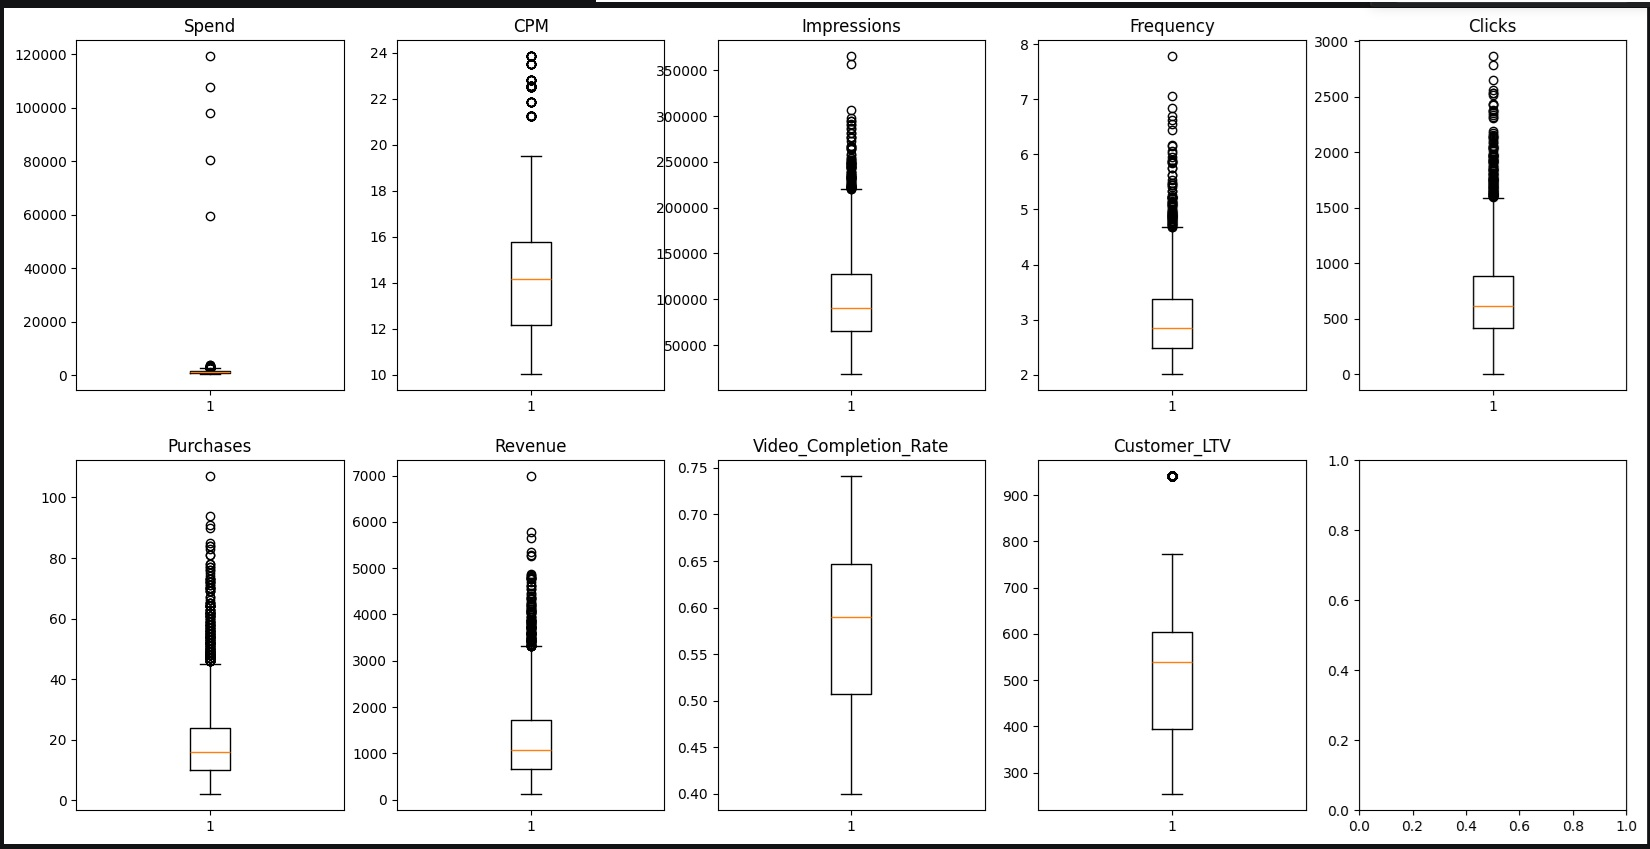
\includegraphics[width=1\textwidth]{images/box_plotsjpg.jpg}
		\caption{Boxplots for all numerical columns of the dataframe}
		\label{fig:box_plots}
	\end{figure}
	
	
	\subsubsection{\texttt{Spend} severe outliers investigation}
	First, I listed the 5 datapoints with severe \texttt{Spend} outliers as shown in \textit{Fig. \ref{fig:spend_outliers}}. I noticed that in this 5 datapoints, the \textbf{CPM do not match the Ad Spend and Impression}. This tells me that there is a possibility that there are more rows with mismatched CPM. 
	
\begin{figure}[h]
	\centering
	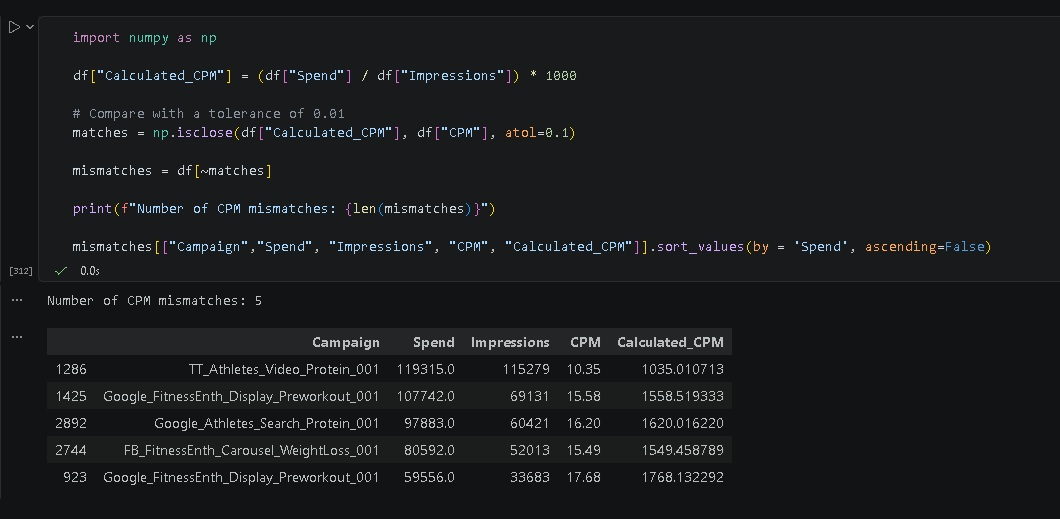
\includegraphics[width=1\textwidth]{images/CPM_mismatch_list.jpg}
	\caption{Number of rows with CPM mismatch}
	\label{fig:CPM_mismatch_list}
\end{figure}	
	
	So, I checked and found out that only these 5 rows have mismatched CPM as shown in \textit{Fig. \ref{fig:CPM_mismatch_list}}, after dropping the rows from earlier(the ones with 0 impression,clicks and purchases).
	
	\begin{figure}[h]
		\centering
		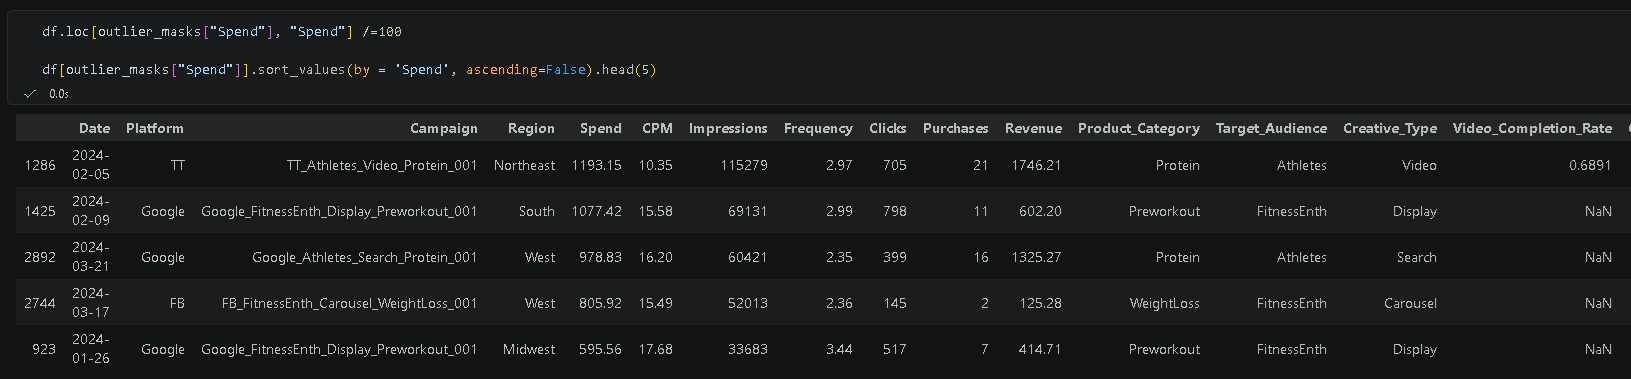
\includegraphics[width=1\textwidth]{images/severe_spend_outlier_list.jpg}
		\caption{Datapoints with severe \texttt{Spend} outliers}
		\label{fig:spend_outliers}
	\end{figure}
	
	Then, I plotted the \texttt{Spend} boxplots of these Campaign Ads.
	
	\begin{figure}[h]
		\centering
		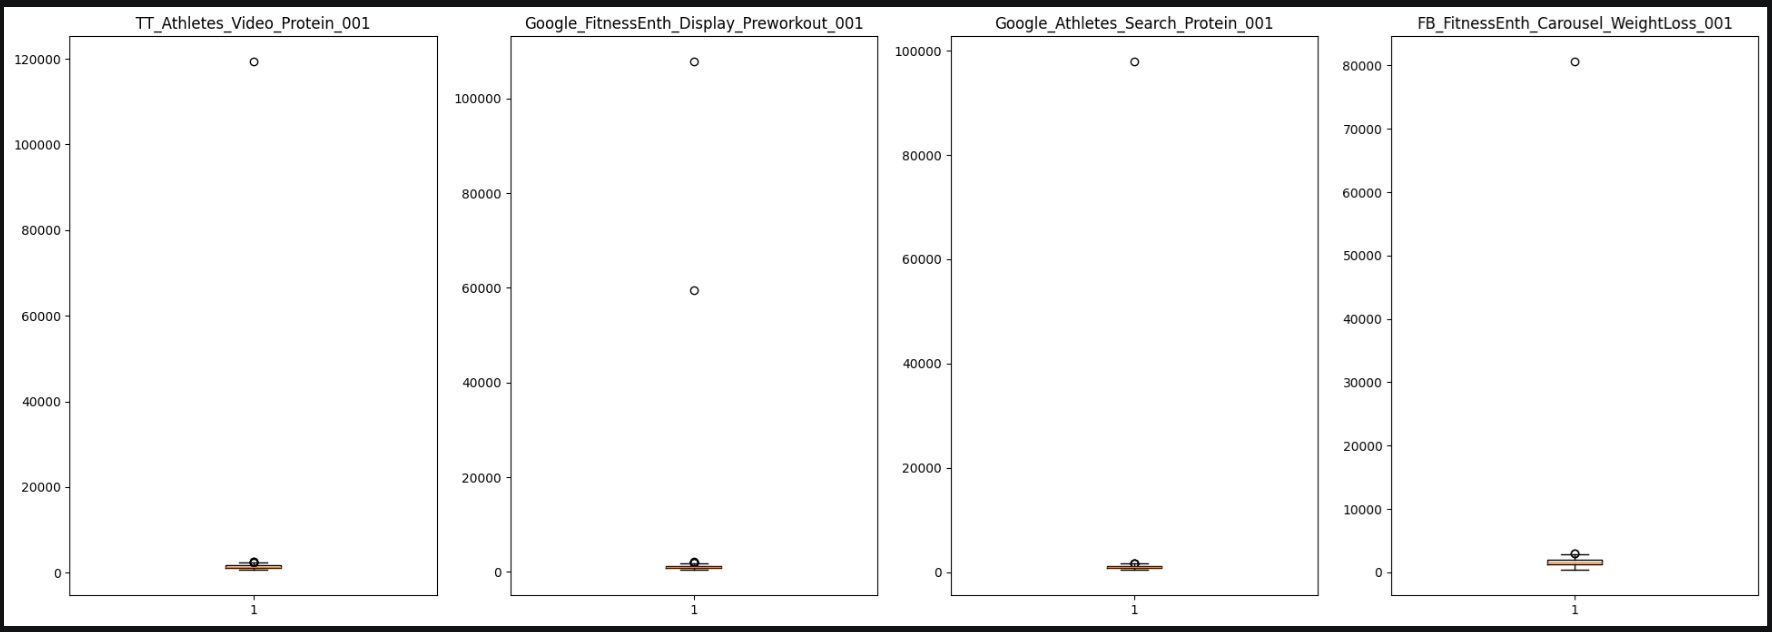
\includegraphics[width=1\textwidth]{images/severe_spend_outlier_boxplot.jpg}
		\caption{\texttt{Spend} boxplots for campaign ads with severe \texttt{Spend} outliers}
		\label{fig:spend_outliers_boxplot}
	\end{figure}
	
	
	From this analysis, I noticed the following consistencies:
	\begin{enumerate}
		\item The reported CPM values(from datapoints with severe \texttt{Spend} outliers) were exactly one-hundredth of the values calculated from the corresponding Spend and Impressions.
		\item The calculated CPM values do not match the `Impressions` and `Spend` columns, and this is limited only to the 5 reported rows with severe `Spend` outliers.
		
		\item Inspection of the affected campaigns showed that the unusually large Spend values occurred only on a single day and were not associated with competitive events.
		
	\end{enumerate}
	Since the discrepancy was systematic (a factor of 100) and limited to these five observations, the Spend values were divided by 100 to restore consistency with the reported CPM values.
	

	
	\subsection{Data Cleaning Summary}
	
	The data cleaning process consisted of:
	
	\begin{itemize}
		\item Verified variable data types
		
		\item Verifying duplicate observations
		
		\item Removing observations(20 datapoints) with missing revenue.
		
		\item Retaining structurally missing Video Completion Rate values.
		
		\item Retaining valid view-through conversions.
		
		\item Removing observations(47 datapoints) with 0 clicks,impressions and purchases with non-zero purchase. 
		
		\item Addressed severe \texttt{Spend} outliers.
		

	
		
	\end{itemize}
	
	Overall, the dataset was determined to be sufficiently complete and reliable for subsequent analysis.
	
